%=================================================================
% G-Code Decoder paper -- two-column IEEE conference version (v5_conference).
% Compile: pdflatex; bibtex decoder_paper_v5_conf_ieee; pdflatex x2
%=================================================================
\documentclass[conference]{IEEEtran}
\IEEEoverridecommandlockouts

\usepackage{cite}
\usepackage{amsmath,amssymb}
\usepackage{siunitx}
\usepackage{multirow}
\usepackage{booktabs}
\usepackage{graphicx}
\usepackage{subcaption}
\usepackage{enumitem}
\usepackage{float}
\usepackage{xcolor}
\usepackage{url}
\usepackage{tikz}
\usetikzlibrary{arrows.meta, positioning, decorations.pathreplacing}
\graphicspath{{../figures/}}

% Custom commands
\newcommand{\modelname}{G-Code Decoder}
\newcommand{\encname}{MM-DTAE-LSTM}
\newcommand{\ie}{\textit{i.e.}}
\newcommand{\eg}{\textit{e.g.}}
\newcommand{\etal}{\textit{et al.}}
\newcommand{\etc}{\textit{etc.}}
\newcommand{\TBD}[1]{\textcolor{red}{\textbf{[TBD: #1]}}}

\begin{document}

\title{Per-Field Categorical G-Code Recoverability from Multi-Modal Sensor Embeddings on a Desktop CNC Mill: A Single-Platform Characterization Study}

\author{%
\IEEEauthorblockN{Stephen S. Eacuello, Romesh S. Prasad, and Manbir S. Sodhi}
\IEEEauthorblockA{Department of Industrial and Systems Engineering\\
University of Rhode Island, Kingston, RI 02881, USA\\
Email: seacuello@uri.edu}
}

\maketitle

\begin{abstract}
Controller-resident tampering can alter executed G-code while the loaded file's hash stays valid. We characterize \textbf{per-field categorical recoverability} of G-code from a desktop CNC mill's 4~Hz seven-modality sensor stream, using a grammar-constrained six-head Transformer decoder over a frozen denoising encoder under five-fold file-level cross-validation. Categorical fields are recoverable under reference-conditioned (teacher-forced) evaluation, the command head at $\sim\!0.89$ accuracy; measured free-running categorical accuracy collapses to $0.48$. The decoder adds $+22$~pp over the history-free operation-class modal ($0.795$ vs.\ $0.572$, command-token positions) and $\approx\!+13$~pp over a history-matched Markov null ($0.662$); the increment is a 4-of-5-fold effect (at or below the class prior on one fold) and an \emph{upper} bound on sensor-driven recovery. By contrast, generative reconstruction collapses: token accuracy falls $0.78\!\to\!0.21$ and digit $0.59\!\to\!0.10$ under autoregression, with whole-sequence exact-match at $0.026$ under exposure-bias mode collapse, on a corpus in which $77.7\%$ of blocks occupy $\le\!1$ sample period. Under open-vocabulary leave-one-class-out evaluation, command recovery collapses to $0.213$. Generative coordinate reconstruction is unsupported (source-entropy and sub-Nyquist bounds; companion paper). Tamper detection is deferred to a companion security study; the posture is forensic-support post-hoc audit in a single-platform, closed-world scope, not real-time intrusion detection.
\end{abstract}

\begin{IEEEkeywords}
CNC machining, G-code reconstruction, multi-modal sensor fusion, manufacturing cybersecurity, tamper detection, grammar-constrained inference, forensic audit
\end{IEEEkeywords}

% =====================================================================
% =====================================================================
\section{Introduction}
\label{sec:introduction}

A Computer Numerical Control (CNC) milling machine drives a cutting tool along G-code toolpaths to micrometer tolerances, and every cut leaves a multi-modal signature in vibration, acoustic emission, motor current, and environmental channels. Whether that signature is informative enough to \emph{recover} the executed instruction stream line by line, without controller access, is the question of this paper. The application is forensic-support post-hoc audit, a controller-independent record of executed instructions, not real-time intrusion detection~\cite{nist2023sp80082,sturm2014cyber,yampolskiy2018security,kimmell2025cnc}. All results are conditional on a single desktop mill (air-cut and UHMW-PE active-cut runs, 4~Hz envelope-extracted stream); cross-platform replication is future work (Section~\ref{sec:roadmap}).

CNC milling is a harder signal environment than the additive-manufacturing side-channel analog~\cite{alfaruque2016acoustic,song2016my,chhetri2016kcad}: simultaneous multi-axis interpolation, nonlinear force engagement, and frame-borne vibration corrupt the signal, and the sensor-to-instruction mapping is many-to-one~\cite{teti2010advanced,wang2018deep}. We take a prior multi-modal denoising encoder (96.3\% nine-class operation accuracy~\cite{encoder_paper}) as a frozen feature extractor and a companion grammar tokenization~\cite{grammar_paper} as vocabulary, and ask what its per-window latent carries about the row-level instructions. Three task-specific obstacles shape the design: a 64-second window straddles many G-code rows, so window-level targets destroy row information; the numeric vocabulary holds thousands of sparse bucket tokens; and positional metadata is a shortcut that inflates accuracy without proving sensor-driven recovery~\cite{meyes2019ablation}.

\paragraph{Headline findings (stated as bounds).} The central quantities are not the closed-vocabulary $\sim\!0.89$ command accuracy but two bounds. Above the operation-class modal predictor, the decoder adds a $+22$~pp class-prior-controlled within-class command increment, an \emph{upper} bound on sensor-driven recovery that is a 4-of-5-fold effect, at or below its class prior on one fold, and $\approx\!+13$~pp against a history-matched sensor-free Markov null (Section~\ref{sec:disc-confound}). On an open-vocabulary leave-one-class-out holdout, command recovery collapses to a floor of $0.213$. End-to-end generative reconstruction is at floor (autoregressive whole-sequence exact-match $0.026$). We reserve ``recovery'' for the per-field categorical heads and treat generative coordinate reconstruction as unsupported on this stack. Because $77.7\%$ of rows occupy $\le\!1$ sample period at 4~Hz, all recovery claims are window-aggregated row-modal, not sub-sample per-row.

\paragraph{Contributions.}
\begin{enumerate}[label=\textbf{(\arabic*)}, leftmargin=*]
\item \textbf{Per-row and full-window supervised targets.} A per-row formulation maps each sensor window to the single G-code line firing within it ($\sim$19{,}500 samples per fold versus $\sim$300 at window level), removing within-window label ambiguity; the headline configuration trains on the full-window variant, which restores within-window row identifiability (Section~\ref{sec:results-rq2}).
\item \textbf{\modelname{} architecture.} A Transformer decoder with six structured heads (token, type, motion-command, parameter-type, sign, digit) over the frozen encoder latent~\cite{encoder_paper}, grammar-constrained so structurally invalid transitions are masked at runtime~\cite{outlines,xgrammar}.
\item \textbf{Per-axis recoverability characterization} reporting, per field, axis detection, motion-direction correctness, and numeric recovery over X, Y, Z, R.
\item \textbf{Ablation matrix} over metadata access, per-row vs.\ full-window targets, seven sensor modalities, and a no-numeric retraining.
\item \textbf{Cross-class generalization study}: leave-one-class-out across nine operation classes, testing memorized per-class shortcuts against within-envelope generalization.
\item \textbf{From-scratch Transformer seq2seq baseline} scoping the architectural lift; a companion limit paper~\cite{paperB_entropy} accounts for why the recoverability pattern takes this shape.
\end{enumerate}

% =====================================================================
\section{Related Work}
\label{sec:related}
\label{sec:related-cnc}\label{sec:related-seq2seq}\label{sec:related-sidechan}\label{sec:related-security}

Sensor-based machining monitoring is mature but coarse-grained: force, vibration, acoustic emission, temperature, and motor current support tool-condition and process assessment~\cite{teti2010advanced,zhu2009wavelet,mohanraj2020tool}, via deep feature learning~\cite{wang2018deep,zhao2019machine} and multi-modal fusion~\cite{lahat2015multimodal,ramachandram2017deep,cao2023crossattention}, but at session- or class-level targets~\cite{tsanousa2022multisensor,stathatos2024cnn,coelho2024anomaly}. Grammar-constrained decoding prunes structurally invalid tokens at inference~\cite{picard,outlines,xgrammar,geng2023gcd}, and G-code fits this treatment~\cite{grammar_paper,gcode_foundational}. The closest analog is additive-manufacturing side-channel toolpath reconstruction from acoustic~\cite{alfaruque2016acoustic,song2016my}, optical~\cite{chattopadhyay2025video}, and acoustic-magnetic~\cite{jamarani2024screg} channels, but at kHz--MHz raw rates rather than our 4~Hz audio-RMS envelope; Kimmell \etal~\cite{kimmell2025cnc} perform binary CNC attack detection, not reconstruction. File-hash signing~\cite{belikovetsky2017drowned} and controller attestation~\cite{zonouz2014plc} are orthogonal non-sensor defenses. To our knowledge this is the first per-instruction, per-field categorical recovery of CNC \emph{milling} G-code from a multi-modal sensor stream; the 5-fold file-level cross-validation and nine-class LOCO protocol support that claim rather than standing as a co-equal novelty leg.\label{sec:related-comparison}

\section{Problem Formulation}
\label{sec:problem}

\subsection{Task Definition}
\label{sec:task}

Let $W \in \mathbb{R}^{T \times C}$ be a sensor window of $T$ samples over $C$ channels aligned to a CNC milling operation, and $g$ the G-code line executing within it. We learn a mapping
\begin{equation*}
  f_\theta: W \mapsto \hat{g}, \qquad \hat{g} = (\hat{t}_1, \hat{t}_2, \dots, \hat{t}_L),
\end{equation*}
producing a length-$L$ token sequence from a vocabulary $\mathcal{V}$. Training minimizes a multi-head cross-entropy loss with the structured heads of Section~\ref{sec:decoder}. At inference the decoder generates tokens autoregressively under a grammar mask that zeros structurally invalid transitions in the legacy-token head.

\subsection{Vocabulary and Token Types}
\label{sec:problem-vocab}

Each motion block is a \emph{rapid move} (\texttt{G0}, traverse) or a \emph{cutting move} (\texttt{G1}/\texttt{G2}/\texttt{G3}, linear and arc feeds); all blocks are tokenized by a hybrid scheme that separates structural primitives from numeric values~\cite{grammar_paper,gcode_foundational}. The vocabulary has four classes: SPECIAL (\texttt{PAD}, \texttt{BOS}, \texttt{EOS}, \texttt{UNK}, \texttt{MASK}); COMMAND (literal motion or machine commands \texttt{G0}, \texttt{M3}, \ldots); PARAM (axis or rate address letters \texttt{X}, \texttt{Y}, \texttt{Z}, \texttt{F}, \texttt{S}, \ldots); and NUMERIC (bucketed values, one bucket per (axis, magnitude) pair). NUMERIC dominates, with 1{,}048 \texttt{NUM\_X}, 1{,}086 \texttt{NUM\_Y}, and 231 \texttt{NUM\_Z} buckets; total vocabulary size 2{,}418. For example, \texttt{G1 X1.4919 Y1.4848 F22.} becomes \texttt{BOS G1 X NUM\_X\_1492 Y NUM\_Y\_1485 F NUM\_F\_22 EOS}.

\subsection{Per-Row Target Formulation}
\label{sec:per-row}

A 256-sample window at 4~Hz spans 64 seconds and averages 60 G-code rows, so a window-level target aggregates across rows and discards row-level distinctions such as an \texttt{X} positive versus negative move. We instead emit one $(W, g_r)$ pair per row $r$ firing within $W$, with $g_r$ that row's token sequence. This removes within-window label ambiguity, raises the training-sample count by an order of magnitude ($\sim$19{,}500 versus $\sim$300 per fold), and blocks positional-shortcut inference on \texttt{(window\_index, source\_file)}. A complementary \emph{full-window} formulation keeps one sample per window with a multi-line target of all fired rows in temporal order. The headline configuration (Table~\ref{tab:headline}) trains on full-window targets, which restore within-window row identifiability (Section~\ref{sec:results-rq2}); per-row targets remain the preferred autoregressive deployment mode, since per-row predictions are short and independent across rows, with the command-head cost of the per-row mode given by the $0.499$-versus-$0.888$ target-mode contrast (Section~\ref{sec:results-rq2}).

\subsection{Evaluation Metrics}
\label{sec:metrics}

We report seven metrics: token accuracy (the headline; fraction of non-padding positions whose argmax matches the target), sequence accuracy (strict exact-match over all non-padding tokens in a sample), and per-token accuracy on the type (4-way), motion-command (6-way), parameter-type (10-way), sign (3-way), and per-digit NUMERIC heads. Macro precision, recall, and F1 follow per head~\cite{pedregosa2011sklearn}.

\paragraph{Teacher-forced vs.\ autoregressive evaluation.} \emph{Teacher-forced} (TF) evaluation supplies the ground-truth previous token at every position (the training objective); \emph{autoregressive} (AR) evaluation consumes the model's own predictions, measuring end-to-end generation when no controller log anchors the sequence. The categorical heads (type, command, parameter-type, sign) are evaluated from the ground-truth-conditioned forward pass in both regimes and therefore carry a single number each; because they read the decoder hidden state, which is computed from the conditioning token stream (Section~\ref{sec:multihead}), their free-running accuracy is distinct and collapses when measured (command $0.483 \pm 0.049$). The autoregressive-token heads score lower under AR because exposure-bias errors compound. The headline table reports both regimes for the token heads.

\subsection{Threat Model (Companion Study)}
\label{sec:problem-threat-model}

The application motivating per-field recoverability is out-of-band verification of the executed instruction stream against controller-resident tampering. The full threat model --- trusted and untrusted elements, the attack-class taxonomy, and per-class detectability --- is developed in a companion security study (in preparation); the present paper characterizes only which G-code fields are recoverable, the precondition for any such monitor.

% =====================================================================
% =====================================================================
\section{Method}
\label{sec:method}

\subsection{System Overview}
\label{sec:system-overview}

\begin{figure*}[!t]
\centering

\includegraphics[width=0.56\linewidth]{system_overview.pdf}
\caption{System overview. A 64-second sensor window ($256$ samples $\times$ $98$ channels across seven modality groups) is mapped by the frozen \encname{} encoder ($\approx$5.1\,M active parameters) to a $256 \times 256$ memory tensor. An 8-layer Transformer decoder ($d_{\text{model}}{=}384$, 12 heads) consumes this memory via cross-attention and generates tokens autoregressively. Six prediction heads share the decoder's hidden state and provide structured output (token, type, motion-command, parameter-type, sign, per-position digit). A static grammar mask zeros structurally invalid token transitions in the legacy-token softmax at inference time.}
\label{fig:system-overview}
\end{figure*}

The system has three stages (Figure~\ref{fig:system-overview}): a frozen multi-modal encoder produces a memory sequence from the sensor window; a Transformer decoder generates the executing G-code line via cross-attention; and a grammar mask zeros structurally invalid softmax transitions at inference. Encoder training is described in~\cite{encoder_paper}.

\subsection{Sensor Encoder (Frozen)}
\label{sec:encoder}

The frozen encoder (\encname{}) is a multi-modal denoising autoencoder over seven modality groups totaling $C=98$ channels, fused by learned modality-weighting gates~\cite{lahat2015multimodal,ramachandram2017deep} and a multi-head self-attention stack~\cite{vaswani2017attention}, with a two-layer LSTM~\cite{hochreiter1997long,malhotra2015lstm} producing the temporal memory. Its $\approx\!5.1$~M active parameters reach 96.3\% test-set accuracy on the nine-class operation-type task~\cite{encoder_paper}, trained on the same file-level 5-fold splits.

\subsection{Decoder Architecture}
\label{sec:decoder}

\modelname{} is an 8-layer Transformer decoder with $d_{\text{model}}=384$ and $h=12$ attention heads per layer, each applying masked self-attention, cross-attention over the encoder memory, a GELU feed-forward network, and pre-layer-norm residuals~\cite{ba2016layernorm} with dropout~\cite{srivastava2014dropout} $0.1$. It has $31.28$~M trainable parameters; with the frozen encoder ($\approx\!5.1$~M active) the total system is $\approx\!36.4$~M.

\subsubsection{Multi-Head Structured Output}
\label{sec:multihead}

Six prediction heads share the decoder's final hidden state at each position, each a linear projection then softmax, trained jointly with a weighted cross-entropy loss:
\begin{equation*}
\begin{aligned}
\mathcal{L}_{\text{decoder}} ={}& \lambda_{\text{tok}}\mathcal{L}_{\text{tok}} + \lambda_{\text{type}}\mathcal{L}_{\text{type}} + \lambda_{\text{cmd}}\mathcal{L}_{\text{cmd}} \\
& {}+ \lambda_{\text{param}}\mathcal{L}_{\text{param}} + \lambda_{\text{digit}}\mathcal{L}_{\text{digit}} + \lambda_{\text{sign}}\mathcal{L}_{\text{sign}}.
\end{aligned}
\end{equation*}
Default weights are $\lambda_{\text{tok}}=3.0$ with all auxiliary $\lambda=1.0$; the auxiliary heads regularize the shared representation toward token-type-aware features. The heads are: the legacy token head, a vocabulary-sized softmax (2{,}418 classes) that is the primary inference output, grammar-masked (Section~\ref{sec:grammar}) before the softmax; a 4-way type head over \{SPECIAL, COMMAND, PARAM, NUMERIC\}; a 6-way motion-command head over \{G0, G1, G2, G3, G53, M30\}; a 10-way parameter-type head over \{X, Y, Z, I, J, K, R, F, S, P\}; a 3-way sign head over \{POSITIVE, NEGATIVE, ABSENT\}; and a six-position 11-way digit head reconstructing each NUM token digit-by-digit. The categorical heads read this shared hidden state, which is computed from the conditioning token stream; the headline categorical values condition on the ground-truth stream, and under free-running generated-stream conditioning the heads collapse (command $0.483 \pm 0.049$; Section~\ref{sec:metrics}).

\subsubsection{Grammar-Constrained Decoding}
\label{sec:grammar}

G-code follows a regular grammar. We encode the local rules as a static $|V| \times |V|$ binary transition mask on the legacy-token logits at each inference step, cutting the valid next-token set from $|V|=$ 2{,}418 to 31.8 tokens on average, following established runtime grammar-mask patterns~\cite{picard,outlines,xgrammar,geng2023gcd}. A separate inference-time FSM layer tracks the most recent move-command and forbids command-state violations the bigram mask cannot express (e.g.\ R/I/J after G0/G1). With the FSM active, command-state (V1) violations drop to $0$ ($100\%$ reduction) at a 5-fold accuracy cost within fold-to-fold noise (paired-$t$ and Wilcoxon $p>0.4$); we adopt it as the default deployment-time configuration. Full counts are in \texttt{audit/fsm\_vs\_bigram\_paired\_stats.json}.

\subsubsection{Scheduled Sampling}
\label{sec:scheduled-sampling}

Teacher forcing is the training default; the headline configuration uses scheduled sampling~\cite{scheduled_sampling} with $p_{\text{max}}=0.5$, which lifts command accuracy $+17$~pp over the $p_{\text{max}}=0$ teacher-forced variant. Because the sweep that selected it touches held-out test metrics, this is a configuration choice, not an independent generalization estimate.

\subsection{Training Configuration}
\label{sec:training}

The decoder is optimized with AdamW~\cite{loshchilov2019adamw} ($\eta = 5 \times 10^{-5}$, weight decay 0.05) for up to 300 epochs with early stopping on validation token accuracy (patience 75), a 10-epoch linear warm-up, batch size 64, and gradient clipping at norm 1.0. The baseline trains \emph{without} positional metadata (Section~\ref{sec:results-rq2} ablates this).
\section{Experimental Setup}
\label{sec:setup}

\subsection{Dataset}
\label{sec:dataset}

The corpus is 120 aligned CSV files from a Bantam Tools desktop CNC mill~\cite{encoder_paper}. Six multi-sensor boards are aligned at an effective 4~Hz rate across seven modalities (accelerometer, gyroscope, magnetometer, RGBA color, temperature [the ablations' ``environmental''], audio RMS, motor current [``electrical'']); after the encoder paper's consistency audit we retain $C=98$ channels, each envelope-extracted to 4~Hz by a single-pole IIR filter that trades kHz-band acoustic-emission content~\cite{teti2010advanced} for a $\sim$1.5~kB/s stream. The nine operation classes cross three motion strategies (face, pocket, adaptive) with three run conditions~\cite{encoder_paper}: standard air-cuts, \texttt{150025} active cuts engaging UHMW-PE at $0.635$~mm depth, and damaged-spindle air-cuts (one drive band removed; \texttt{audit/operation\_class\_inventory.json}). All runs execute dry on one low-amplitude, stepper-driven platform; whether the factorization transfers to a production VMC is open.

\subsection{Preprocessing and Windowing}
\label{sec:preprocessing}

Sliding windows of $T=256$ samples (64~s at 4~Hz) at stride 64 are aligned to their overlapping G-code rows. The per-row target formulation emits one $(W, g_r)$ pair per row firing within window $W$, yielding $\sim$19{,}500 training pairs per fold; the headline configuration trains on the full-window variant (Section~\ref{sec:per-row}). The 4~Hz rate constrains recoverability. A row-execution audit (\texttt{audit/gcode\_row\_durations.json}) shows $77.7\%$ of row instances occupy $\le$1 sample period, against the $\geq$10~kHz of conventional tool-condition monitoring~\cite{teti2010advanced}.

\subsection{Five-Fold File-Level Stratified Cross-Validation}
\label{sec:cv}

File-level stratified five-fold cross-validation prevents within-file leakage, and each fold covers all nine classes. A G-code-line coverage-repair step swaps files between train and test until every test line also appears in training, constructing a closed-vocabulary regime ($97.6\%$ of distinct test lines, $99.0\%$ of instances seen verbatim). The headline numbers are therefore within-vocabulary classification, not open-vocabulary recovery; the matched open-vocabulary number is the leave-one-class-out (LOCO) command accuracy of $0.213 \pm 0.191$ (Section~\ref{sec:loco}). Overlapping windows ($75\%$ overlap) make adjacent within-file windows non-independent, so we take the per-fold mean as the unit of analysis.

\subsection{Statistical Analysis}
\label{sec:stats}

For each five-fold ablation we report the cross-fold mean and standard deviation, with $n=5$ per group. All $p$-values are \emph{descriptive} and the bootstrap 95\% intervals a smoothed, not coverage-calibrated, indication of cross-fold spread; conclusions rest on effect sizes large relative to that spread rather than on significance thresholds, with nonparametric (Wilcoxon) checks accompanying the paired tests where reported. Single-fold pilots are excluded from quantitative claims; the leave-one-class-out protocol (Section~\ref{sec:loco}), though single-fold per holdout, is reported as a finite-population descriptive result over the nine-class corpus.

\subsection{Software and Compute}
\label{sec:software}

The decoder is implemented in PyTorch and trained on NVIDIA RTX A6000 GPUs; preprocessing uses scikit-learn~\cite{pedregosa2011sklearn} and SciPy~\cite{virtanen2020scipy}, with full code and configuration released with the manuscript.

% =====================================================================
% =====================================================================
\section{Results}
\label{sec:experiments}

\subsection{Non-Neural Baseline Comparison}
\label{sec:results-baseline}

Two lightweight classifiers on the mean-pooled encoder embedding the decoder consumes, a scikit-learn \texttt{HistGradientBoosting} (HGB) tree-booster and a two-layer MLP probe, hit the class-prior ceiling on the binary fields ($\approx\!0.88$ \emph{has-X}, $0.99$ \emph{has-F}) but fall to macro-F1 $0.23$--$0.25$ on multi-class command identity; HGB reaches macro-F1 $0.86$ on the one within-window-diverse field \emph{has-Z}, so the pooled embedding carries some per-row Z signal (fold-1 reference on per-row targets; \texttt{audit/nonneural\_baselines.json}).

\subsection{Headline Accuracy and Per-Field Recoverability}
\label{sec:results-headline}

Table~\ref{tab:headline} reports headline accuracies per head across five folds under teacher-forced (TF) and autoregressive (AR) evaluation. The categorical heads, each reported from the ground-truth-conditioned pass (free-running they collapse, command $0.483$; Section~\ref{sec:metrics}), reach type $0.9838$, command $0.8875 \pm 0.0558$, parameter-type $0.9931$, and pooled motion-sign $0.9888$. The autoregressive-token heads diverge sharply: token accuracy $0.7811$ (TF) versus $0.2148$ (AR), numeric $0.5850$ (TF) versus $0.1038$ (AR). Sequence exact-match, defined only under AR, is $0.0263 \pm 0.0185$, fewer than $3\%$ of windows reproduced verbatim; it is the deployment-relevant generative figure. The TF--AR gap is the exposure-bias signature of autoregressive mode-collapse (analyzed in the extended version of this work), and the headline is seed-robust (four seeds span $0.0085$, Appendix~\ref{app3:repro}). A float-epsilon artifact at the finest decimal slot was corrected by a round-encoding retrain; headline and categorical metrics drift $\le\!1.5$~pp under it, so Table~\ref{tab:headline} uses the released checkpoint and the patched retrain serves only the numeric tier (Section~\ref{sec:numeric-decomposition}).

We reserve \emph{recovery} for the per-field categorical heads (command, parameter-type, sign) under reference-conditioned evaluation. End-to-end generative reconstruction is at floor, so this paper claims per-field categorical recoverability, not toolpath reconstruction. Command macro-F1 is $0.879$, moderately below accuracy on the long-tailed class distribution, with recovery across all six classes and no collapse (lowest G2 at $0.82$; per-class F1 in the extended version); parameter-type macro-F1 is $0.986$.

Three caveats bound these numbers. They are closed-vocabulary, in-distribution ($97.6\%$/$99.0\%$ verbatim test-line overlap), so command $0.8875$ is within-vocabulary classification, not an open-vocabulary deployment number. The frozen encoder shared the file-level fold partitions, so the headline carries a representation-reuse component bounded in Appendix~\ref{app3:addenda}. The LOCO cross-class command accuracy of $0.213 \pm 0.191$ (Section~\ref{sec:loco}) is the open-vocabulary floor.

% Headline 5-fold metrics. Reports both teacher-forced (TF, sweep-time) and
% autoregressive (AR, deployment-true) numbers per head. Categorical heads
% carry a single reference-conditioned value; measured free-running AR
% categorical accuracy collapses (command 0.483, type 0.551, param-type 0.533;
% audit/ar_categorical_freerunning.json, see footnote). The autoregressive-token
% heads (token, sequence, numeric) drop under AR due to exposure bias.
\begin{table*}[!t]
\centering
\caption{Headline test-set metrics for the G-Code Decoder under 5-fold file-level cross-validation, full-window targets, no positional metadata exposed. Mean $\pm$ std over 5 folds. Two evaluation regimes are reported: teacher-forced (TF), where each step receives the ground-truth previous token, and autoregressive (AR, greedy / beam-width 1), where the decoder consumes its own previous predictions. The categorical heads --- type, command, parameter-type, sign --- report a single reference-conditioned value (the AR column is marked `--'); measured free-running categorical accuracy is reported in the footnote. Only the autoregressive-token heads (token, sequence, numeric) carry distinct TF and AR values.}
\label{tab:headline}
\resizebox{0.77\textwidth}{!}{%
\begin{tabular}{l r r r r}
\toprule
Head & TF Accuracy & AR Accuracy & Macro Precision & Macro F1 \\
\midrule
Token       & $0.7811 \pm 0.0216$ & $0.2148 \pm 0.0685$ & $0.4099 \pm 0.0406$ & $0.3899 \pm 0.0405$ \\
Sequence$^{\ddagger}$ & -- & $0.0263 \pm 0.0185$ & --                  & --                  \\
Type        & $0.9838 \pm 0.0085$ & --                  & $0.9091 \pm 0.0352$ & $0.8833 \pm 0.0451$ \\
Command     & $0.8875 \pm 0.0558$ & --                  & $0.9342 \pm 0.0407$ & $0.8790 \pm 0.1084$ \\
Param-type  & $0.9931 \pm 0.0036$ & --                  & $0.9914 \pm 0.0073$ & $0.9857 \pm 0.0130$ \\
Sign        & $0.9888 \pm 0.0063$ & --                  & $0.9658 \pm 0.0215$ & $0.9724 \pm 0.0157$ \\
Numeric (overall digit) & $0.5850 \pm 0.0331$ & $0.1038 \pm 0.0322$ & --      & --                  \\
\bottomrule
\end{tabular}%
}
\par\smallskip
\footnotesize\textit{Macro precision and F1 are unweighted means over all observed classes; the categorical heads carry a single (reference-conditioned) value. Numeric is the digit-head accuracy pooled across all six digit positions; the per-position bathtub is characterized in Section~\ref{sec:numeric-decomposition}. The TF / AR gap on the token and numeric heads is the exposure-bias signature; the categorical AR column is marked `--' because those values are reference-conditioned; measured free-running categorical accuracy collapses (command $0.483 \pm 0.049$, type $0.551 \pm 0.087$, parameter-type $0.533 \pm 0.046$; \texttt{audit/ar\_categorical\_freerunning.json}). $\ddagger$~Sequence exact-match is reported only under AR; a sequence-level TF score is not separately well-defined (see Section~\ref{sec:results-headline}).}
\end{table*}


\subsection{Per-Axis Recoverability}
\label{sec:per-axis}

For each axis letter we score \emph{has-axis} (axis present in the predicted block), \emph{sign} (motion sign when present), and \emph{value MAE} (mean absolute error where both blocks carry the axis); near-zero-presence fields cannot be meaningfully evaluated (Table~\ref{tab:per_axis}).

\input{../tables/per_axis_recoverability_ieee.tex}

\begin{figure*}[!t]
\centering
\begin{subfigure}{0.40\linewidth}\centering
  
\includegraphics[width=\linewidth]{per_axis_recoverability.pdf}
  \caption{Per-axis recoverability (5-fold mean): has-axis F1, motion-sign accuracy, and value MAE (inches). The Y-vs-Z sign asymmetry reflects the near-deterministic Y prior versus Z's balanced sign distribution~\cite{paperB_entropy}.}
  \label{fig:per_axis}
\end{subfigure}\hfill
\begin{subfigure}{0.46\linewidth}\centering
  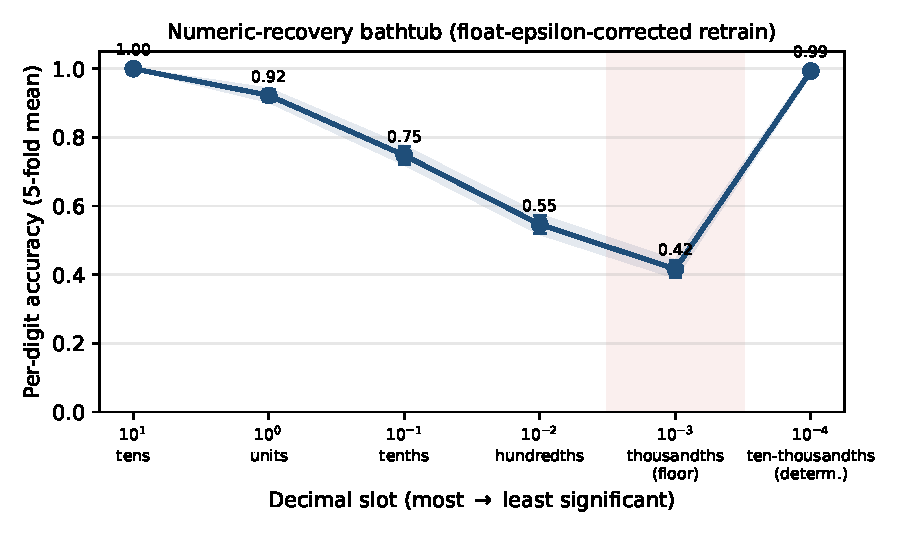
\includegraphics[width=0.8\linewidth]{per_digit_position_curve.pdf}
  \caption{The numeric-recovery ``bathtub'' (per-digit accuracy, 5-fold mean $\pm$ std, teacher-forced, patched retrain): slot~0 at $1.00$ descends to the precision floor at slot~4 ($0.42$, thousandths, the finest tokenizer-retained digit); slot~5 returns to $0.99$ as a structural zero of the V8 tokenizer's $0.001$ grid (discarding the $\sim\!3.31$-bit source digit), not information-bearing recovery~\cite{paperB_entropy}. Source: \texttt{audit/patched\_numeric\_analysis.json}.}
  \label{fig:per_digit_position_curve}
\end{subfigure}
\caption{The numeric tier: per-axis summary (left) and per-digit decomposition (right).}
\label{fig:numeric-tier-pair}
\end{figure*}

Four patterns emerge. Axis-presence detection is uniformly high: X, Y, Z at $1.000 \pm 0.000$, R at $0.994$, and F at $0.960$ on thin support. Motion-sign recovery is axis-asymmetric but \emph{prior-driven}, not a sensor-separability ranking: Y-sign ($0.997$) and X-sign ($0.942$) ride near-deterministic priors, while Z-sign ($0.938$), the only balanced-distribution sensor-bearing axis, scores lower as a harder sensor-driven binary classification, not weaker coupling. Value MAE is small for Z ($0.009$ patched) and arc-radius R ($0.021$) but larger for X ($0.248$) and Y ($0.205$), all in inches, localized to middle digits by the per-digit decomposition. Spindle (S) and arc parameters (I, J) have effectively zero positive support and cannot be evaluated (Figure~\ref{fig:numeric-tier-pair}).

\subsection{Numeric Digit Head Decomposition}
\label{sec:numeric-decomposition}

Per-slot TF accuracy on the corrected retrain is bathtub-shaped (Figure~\ref{fig:per_digit_position_curve}): slot~0 (tens) at $\sim\!1.00$ descends to the \emph{true precision floor} at slot~4 ($0.42$, thousandths, the finest digit the V8 tokenizer retains~\cite{paperB_entropy}). Slot~5 returns to $0.99$ because the V8 tokenizer (the hybrid vocabulary of Section~\ref{sec:problem-vocab}) quantizes X/Y/Z onto a $0.001$ grid, making the tokenized ten-thousandths digit structurally near-zero entropy, deterministically reproduced rather than information-bearing~\cite{paperB_entropy}. The decoder therefore behaves as a coarse-resolution coordinate recoverer, tracking the corpus per-(axis, slot) source-entropy ceiling (corrected pooled Pearson $-0.89$).

\subsection{Per-Operation-Class Recoverability}
\label{sec:per-op-class}

Autoregressive predictions stratify sharply by operation class from a single mechanistic cause: \texttt{face} reaches token $0.56$ / numeric $0.40$ while every other class sits in a narrow $0.09$--$0.25$ token band, because the corpus-modal AR output the decoder collapses to \emph{is} a facing-pattern toolpath, so \texttt{face} scores by coincidental agreement, not per-class capability (per-class figure in the extended version).

\subsection{Metadata, Target-Mode, and Numeric-Collapse Ablations (Extended Version)}
\label{sec:results-rq2}

Three ablations refine the headline and are reported in full in the extended journal version of this work (in preparation): positional metadata does not improve the categorical heads under any regime but mitigates autoregressive mode-collapse ($+7.5$--$8.0$~pp on the AR token/numeric heads); the full-window target formulation lifts command accuracy from per-row $0.499$ to $0.888$ by restoring within-window row identifiability; and a no-numeric retraining decomposes the AR collapse into a numeric-desynchronization component and a dominant intrinsic structural-stream collapse.

\subsection{Sensor-Modality Ablation}
\label{sec:abl-sensors}

For each of seven sensor modality groups (accelerometer, gyroscope, magnetometer, environmental, color, audio-RMS, electrical) we zero the corresponding channels at the encoder input and evaluate without retraining, a \emph{lower bound} on each modality's value. Every modality is critical to the command head at a statistically uniform magnitude: zeroing any single group drops command accuracy from the full-modality baseline $0.888 \pm 0.056$ to the $0.449$--$0.484$ band, a uniform $-40$ to $-44$~pp collapse. The seven-group ANOVA is \emph{not} significant ($F=0.07$, $p=0.998$), while every modality-versus-baseline contrast \emph{is} ($p<0.001$); this confirms joint necessity but cannot rank importance. The coarse heads are more robust (token $\sim\!4$~pp, type $<\!1$~pp, parameter-type $\sim\!1.5$~pp). Table~\ref{tab:sensor_ablation} reports the per-modality numbers.

\input{../tables/sensor_ablation_ieee.tex}

The frozen-encoder ``joint necessity'' is a gating artifact: the encoder routes command-discrimination signal through every modality at once, so zeroing any one degenerates the representation to one sufficient for the coarse heads but not command; a genuine ranking needs the retraining below.

\subsubsection{Per-Modality Encoder Retraining (Leave-One-Modality-Out)}
\label{sec:abl-lomo}

We retrain the encoder from scratch on the $98$-feature base with each modality removed, train a fresh decoder on the resulting frozen encoder, and score all seven cells against a retrained full-stack baseline on a byte-identical held-out split. The retrained baseline reaches command accuracy $0.904 \pm 0.039$, and every removal lands within $\pm 0.013$; the fold-blocked ANOVA is non-significant ($F=0.91$, $p=0.499$) and the Holm-corrected paired test rejects none ($0/7$). Token and numeric heads behave the same. Figure~\ref{fig:lomo_modality} charts the paired deltas against the frozen collapse.

\begin{figure}[!htbp]
\centering
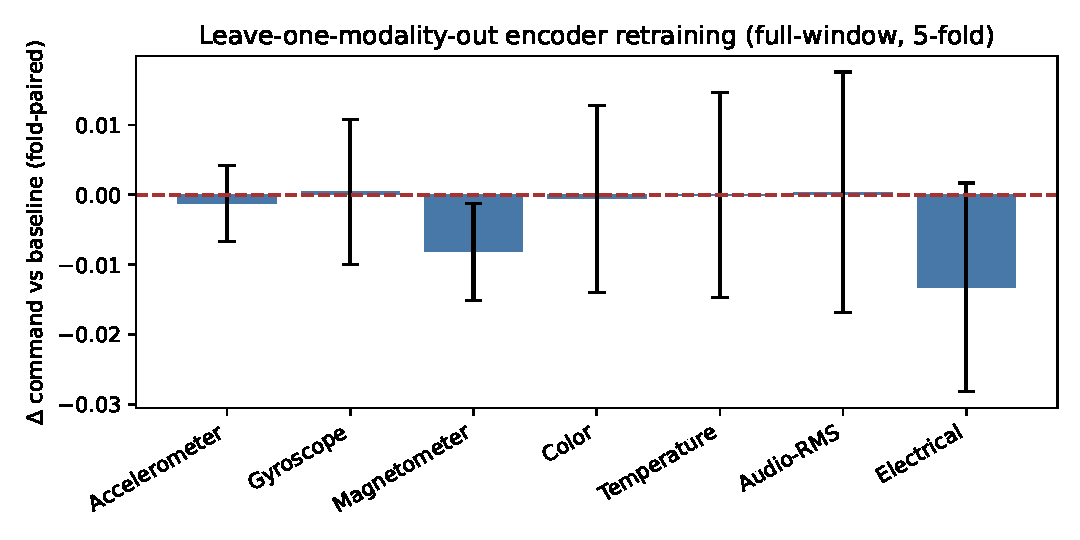
\includegraphics[width=0.5\linewidth]{lomo_modality_bars.pdf}
\caption{Leave-one-modality-out encoder retraining: per-modality fold-paired $\Delta$ command vs.\ the retrained baseline; every modality within $\pm 0.013$, none Holm-significant (fold-blocked ANOVA $F=0.91$, $p=0.499$). Contrast the $-42$~pp uniform collapse under \emph{frozen}-encoder inference-time zeroing (Table~\ref{tab:sensor_ablation}): the gap is the encoder's re-allocation capacity, not modality information content.}
\label{fig:lomo_modality}
\vspace{-6pt}
\end{figure}

The $-42$~pp frozen-encoder collapse reduces to $\le\!1.3$~pp under retraining (none significant), confirming the gating artifact: retraining reallocates capacity onto the remaining channels. The deployment statement upgrades from \emph{``the full multi-modal stack is required''} to \emph{``no single modality is individually load-bearing.''} \label{sec:abl-lomo-sensor-stub}Two orthogonal probes corroborate this: per-board leave-one-sensor-out (LOSO) removals cost $\le\!2.6$~pp (fold-blocked ANOVA $p=0.415$; $0/6$ Holm-significant) and the nested $6\!\times\!6$ (board $\times$ modality) interior is flat within $\pm 0.022$ ($p=0.896$); the redundancy is dense, not a marginal-average effect.

% =====================================================================
\subsection{Cross-Class Generalization (Leave-One-Class-Out)}
\label{sec:loco}

For each of the nine operation classes we train the decoder without that class and evaluate on its held-out samples, testing cross-operation generalization versus per-class memorization. Each holdout re-stratifies the remaining $8$-class fold-1 partition at the headline $80/20$ split (fold~1 is also the covariate-shift outlier of Section~\ref{sec:lim-covariate}, so the LOCO numbers are conditional on this partition choice); the coverage-repair step is deliberately \emph{not} re-run, leaving the open-vocabulary residual exposed. The nine classes are the corpus population, so we report the finite-population descriptive distribution and make no wider inferential claim; each holdout is single-fold.

Across the nine holdouts, command accuracy collapses to mean $0.213$ (min $0.000$, median $0.21$, max $0.678$; $\sigma=0.191$), token to $0.501$, and numeric to $0.152$; type and parameter-type survive ($0.883$ and $0.945$). Relative to the in-distribution 5-fold baseline ($0.888$ command), this is a $\sim\!67$~pp descriptive gap, not a two-sample test: file-stratified CV and class enumeration are different designs, and the per-cell command ranges do not overlap. Eight of nine holdouts cluster in $[0.000, 0.273]$; \texttt{damagepocket} reaches command $0.678$ because it shares its predominantly-G1 motion vocabulary with the retained \texttt{pocket} variants, while \texttt{damageadaptive} ($0.000$) and \texttt{damageface} ($0.094$) do not. Cross-class generalization therefore succeeds only when the held-out class shares motion vocabulary with retained classes. The deployment-realistic claim is bounded by these LOCO numbers, not the 5-fold headline, and is scoped to closed-world audit over the operation classes seen at training time; open-world deployment is out of scope (Section~\ref{sec:future}). Figure~\ref{fig:loco_per_holdout} charts the per-holdout, per-head breakdown.

\begin{figure}[!htbp]
\centering
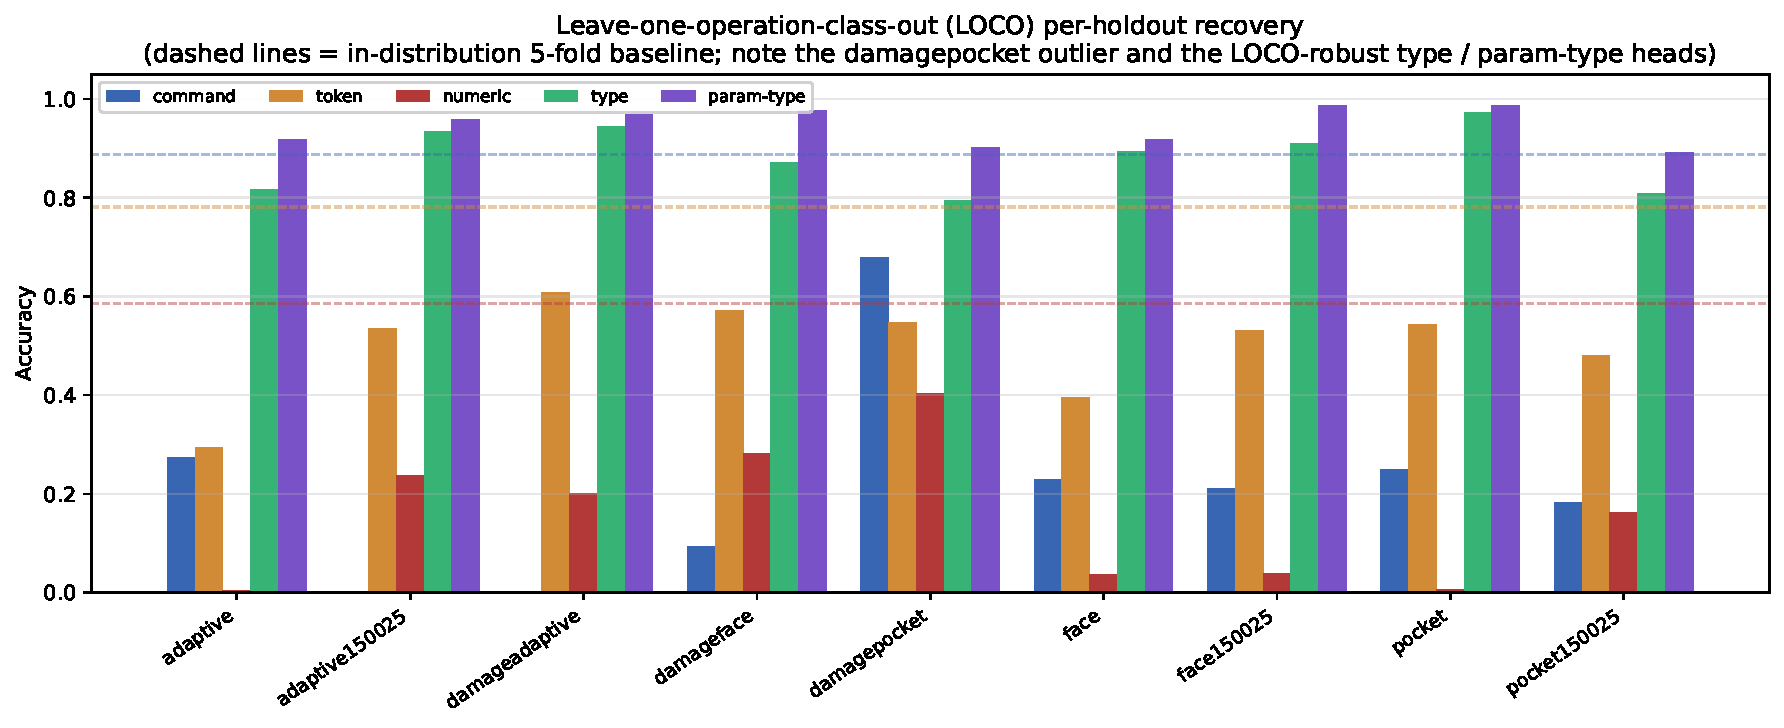
\includegraphics[width=0.5\linewidth]{loco_per_holdout.pdf}
\caption{Leave-one-class-out recovery per held-out class: command/token/numeric/type/parameter-type accuracy; dashed lines are the in-distribution 5-fold baselines. Eight of nine holdouts collapse on command ($\le 0.28$); \texttt{damagepocket} ($0.68$) shares motion vocabulary with retained \texttt{pocket} variants. Type and parameter-type stay near baseline throughout.}
\label{fig:loco_per_holdout}
\vspace{-6pt}
\end{figure}

\subsection{From-Scratch Seq2Seq Baseline (Extended Version)}
\label{sec:abl-seq2seq-baseline}

A from-scratch Transformer seq2seq baseline matches the headline teacher-forced command accuracy ($0.877 \pm 0.031$ vs.\ $0.888 \pm 0.056$) and exceeds its teacher-forced numeric accuracy ($0.754$ vs.\ $0.585$, an advantage that does not survive autoregression), but collapses to the most-frequent-class prior under AR; the extended version shows the apparent AR categorical gap reflects the conditioning-regime difference (reference-conditioned $0.888$ vs.\ measured free-running $0.483$, still above the baseline's AR-derived $0.122$), with the categorical heads carrying the audit-mode signal when a reference stream conditions the decoder.
\section{Discussion}
\label{sec:discussion}

\subsection{What is recoverable, and the class-prior boundary}
\label{sec:disc-deployment}

Recoverability factorizes into three structural tiers (Section~\ref{sec:results-headline}, Table~\ref{tab:per_axis}). Categorical structure (command and axis identity) is strongest: the sensor pathway fixes the motion class and the axes involved independently of file position, and positional metadata adds nothing (Section~\ref{sec:results-rq2}). Motion sign follows, with a prior-driven axis asymmetry (Y near-perfect, X and Z lower). Numeric precision is the limiting tier: a 64-second window observes relative motion, not absolute machine coordinates, so loss concentrates at the fine-value digits (Section~\ref{sec:numeric-decomposition}).

\paragraph{Is categorical recovery sensor-driven or operation-class structure?}\label{sec:disc-confound} The frozen encoder was trained for nine-class operation classification on the \emph{same} fold partitions used here, so the headline command accuracy could be operation-class structure re-expressed at the command level. A class-prior control (\texttt{audit/confound\_class\_prior.json}) tests this at every command-token position: the decoder reaches $0.795 \pm 0.121$ (5-fold) against an operation-class modal null of $0.572$, the strictest legitimate history-free sensor-independent baseline since each test file is unseen. The decoder's figure is measured under teacher forcing with ground-truth within-window history; a sensor-free per-class Markov-1 null granted the same history reaches $0.662 \pm 0.004$ (\texttt{audit/markov\_command\_null.json}), so the history-matched increment is $\approx\!+13$~pp. The $0.795$ is measured only at command-token positions of the full-window predictions, a different position subset and aggregation than the $0.8875$ head accuracy of Table~\ref{tab:headline}; the two are consistent measurements of the same predictions, not a discrepancy. The $+22$~pp increment is a 4-of-5-fold effect, not a uniform one: fold~1 (the covariate-shift outlier, Section~\ref{sec:lim-covariate}) is at or below its class prior, while folds 2--5 sit $+0.27$ to $+0.30$ above (paired-by-fold mean $+0.222$; bootstrap 95\% CI $\approx[+0.10,+0.29]$). At $n\!=\!5$ we report it as an effect size, not a $p$-value. Re-deriving the class-modal null on the test split instead of the training split does not shrink it ($0.576$ vs.\ $0.572$), so roughly $0.57$ of the $0.79$ is prior structure and the decoder adds a within-class increment on top. That increment is an \emph{upper} bound (closed-vocabulary regime, frozen-encoder representation reuse) but unchanged under the test-derived class-modal null.

\subsection{Sensor-stack redundancy and deployment recommendations}
\label{sec:disc-deployment-stack}

\paragraph{Sensor-modality importance.}\label{sec:disc-modality} Under the frozen encoder, inference-time modality removal collapses command accuracy uniformly (between-modality $p\!=\!0.998$), but encoder-retraining LOMO/LOSO ablations (Section~\ref{sec:abl-lomo}) show no single modality or sensor board is individually load-bearing: expected cost is $\le\!1.3$~pp per modality and $\le\!2.6$~pp per board. A cost-reduced post-hoc audit installation is therefore viable on this platform.

\subsection{Security Implications and the Companion Threat-Model Study}
\label{sec:disc-threat-model}

The per-field recoverability characterized here bounds what a sensor-side integrity monitor can and cannot see: categorical substitutions (command, axis, motion-sign) leave a recoverable trace, while numeric-coordinate and feed-rate edits do not (Section~\ref{sec:per-axis}). A companion security study (in preparation) develops the corresponding tamper-detection operating points, alert-budget analysis, and adaptive-adversary bounds under the same closed-world, single-platform scope; those results are reported separately so that this paper's claims rest on recoverability alone.

% =====================================================================
\section{Limitations and Future Work}
\label{sec:future}\label{sec:lim-dataset}\label{sec:lim-method}\label{sec:lim-power}\label{sec:lim-covariate}\label{sec:roadmap}

Every recoverability claim is conditional on one desktop CNC platform and one workpiece material; cross-platform replication on a production-class VMC is the prerequisite for any deployment claim and the principal open direction. Feed rate, spindle speed, and arc parameters have negligible corpus support, so their Table~\ref{tab:per_axis} accuracies are artifacts of near-zero baseline, not sensor-driven recovery. The 4~Hz stack aliases $77.7\%$ of rows into a single sample period, capping numeric precision independently of the sequence head; a higher-rate stack with row-level encoder supervision is the main future direction. The file-level 5-fold splits are closed-vocabulary (every test line was seen in its fold's training), and the open-vocabulary evidence is the leave-one-class-out protocol, under which command accuracy degrades from $0.888$ to $0.213$. A per-field covariate-shift audit flags fold~1 as the outlier fold (modest, $<\!6$~pp shifts on low-support fields; \texttt{audit/extended\_rigor\_audits.json}), the basis for the fold-1 conditionality noted in Sections~\ref{sec:results-headline} and~\ref{sec:loco}.

% =====================================================================
\section{Conclusion}
\label{sec:conclusion}

We characterize which components of an executing G-code block are recoverable from multi-modal CNC sensor data, using \modelname{}, a six-head Transformer decoder on a frozen multi-modal encoder with grammar-constrained inference under five-fold file-level cross-validation. Three findings follow. (1)~\textbf{Per-block categorical recovery} (command, axis, motion direction) is sensor-driven under reference-conditioned evaluation (free-running it collapses to $0.483$): command accuracy is $0.888$, and the class-prior-controlled increment is unchanged under a test-derived class-modal null and $\approx\!+13$~pp against a history-matched Markov null (Section~\ref{sec:disc-confound}); on an \emph{unseen} operation class it collapses to the open-vocabulary floor of $0.213$ (Section~\ref{sec:loco}). (2)~\textbf{End-to-end token and numeric reproduction is at floor}: token accuracy falls from $0.7811$ (TF) to $0.2148$ (AR), numeric from $0.5850$ (TF) toward floor, and whole-sequence exact-match is $0.0263$, bounded by exposure-bias mode-collapse and 4-Hz aliasing atop an information-theoretic limit the companion limit paper~\cite{paperB_entropy} characterizes. (3)~\textbf{Sensor-stack redundancy} is dense ($\Delta\!\le\!2.6$~pp per board), enabling a cost-reduced post-hoc audit installation. The forensic-support post-hoc audit posture is the boundary within which these results hold, not real-time SOC alerting.

% =====================================================================
\appendices
\section{Specification Addenda}
\label{app3:addenda}\label{app:spec-addenda}

The coverage-repair procedure swaps files until every test line also appears in its fold's training partition, converging in $0$--$3$ swaps per fold (assignment released as \texttt{audit/file\_fold\_assignment.csv}). The grammar tokenizer quantizes each axis to a fixed per-axis precision (X/Y/Z at $10^{-3}$) with sign carried by a separate head; empirical bucket counts sum to $K\!=\!2{,}418$, and any out-of-range test index falls back to \texttt{UNK} (closed-vocabulary regime). Representation reuse is bounded two ways: class-label leakage caps the leakage component of command accuracy at $0.572$, and a leave-decoder-test-files-out LOMO-baseline check bounds the empirical reuse effect at $|\Delta|\!\le\!0.016$ ($0.904 \pm 0.039$ vs.\ headline $0.888$).

% =====================================================================
\section{Relationship to the Companion Contributions and Data Availability}
\label{app:companion}

This study is one of four related contributions: an encoder paper~\cite{encoder_paper} establishing the multi-modal denoising sensor encoder and its $96.3\%$ nine-class operation accuracy, a grammar paper~\cite{grammar_paper} defining the hybrid G-code tokenization, the present per-row recoverability characterization, and a companion limit paper~\cite{paperB_entropy} deriving the decoder-agnostic information-theoretic and 4~Hz sub-Nyquist floor that bounds it. Beyond these four, a security companion (in preparation) develops the deferred tamper-detection operating points, and an extended journal version reports the full ablation matrix. The 120-file corpus, per-fold arrays, prediction JSONs, and audit artifacts are released (Data Availability Statement); nothing required to reproduce these results depends on the companion contributions.

% =====================================================================
\section{Reproducibility}
\label{app3:repro}

Training uses AdamW ($\eta=5\times10^{-5}$, weight decay 0.05, batch 64, up to 300 epochs, patience 75) at seed~42; the headline command accuracy is seed-robust (four-seed 5-fold means within a $0.0085$ span, far inside the $\pm 0.0558$ cross-fold spread; \texttt{audit/seed\_robustness\_full\_window.json}). The full hyperparameter grid, per-modality retraining protocol, and statistical exhibits are in the released artifacts (Data Availability).

% =====================================================================

% =====================================================================
\section*{Data Availability}
Sensor datasets, analysis code, per-fold splits, checkpoints, and every cited \texttt{audit/*.json} artifact are publicly available at \url{https://github.com/stephenseacuello/gcode_fingerprinting} (release \texttt{v1.0-submission}; Zenodo DOI in the repository \texttt{README}; code MIT, corpus CC~BY~4.0).

\section*{Acknowledgment}
The authors thank the University of Rhode Island Department of Industrial and Systems Engineering for laboratory and computational resources.

% =====================================================================
\bibliographystyle{IEEEtran}
\bibliography{decoder_references_ieee.bib}

\end{document}
